\section{temp}
\subsection{Visitor Pattern}
\begin{frame}{Traversing the Tree}
\framesubtitle{Visitor Pattern}
	\begin{itemize}
        \item ANTLR visitor pattern
        \item Our own Visitor Pattern
    \end{itemize}
    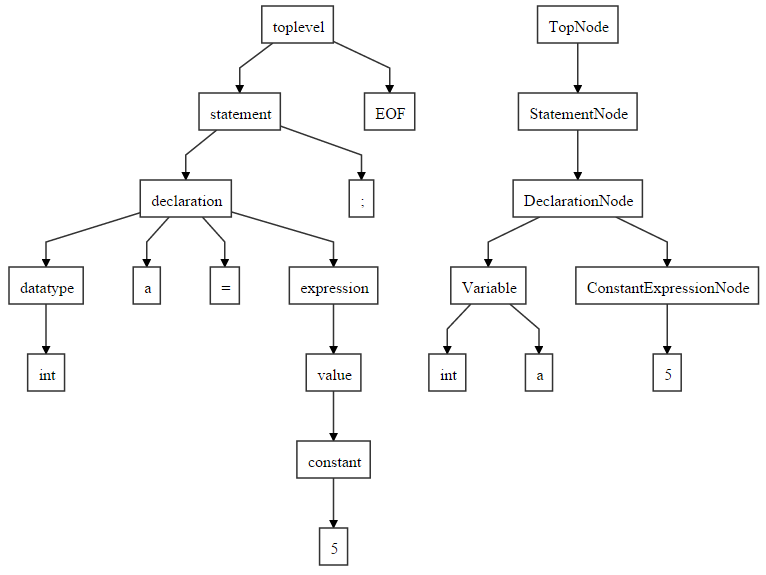
\includegraphics[width=1\textwidth,height=0.7\textheight,keepaspectratio, , clip]{images/P4/AST.PNG}

\end{frame}

\begin{frame}{Contextual Analysis}
\framesubtitle{Module call}

    \begin{lstlisting}
ContextualAnalyser contextualAnalyser = new ContextualAnalyser(inputFile, errors);
abstractSyntaxTree = contextualAnalyser.GenerateDecoratedASTFromParseTree(abstractSyntaxTree);
    \end{lstlisting}


\end{frame}

\begin{frame}{Contextual Analysis}
\framesubtitle{Module call}

\begin{lstlisting}
public BaseASTNode GenerateDecoratedASTFromParseTree(BaseASTNode abstractSyntaxTree){

  //Add potential imported function declarations
  handleImports(abstractSyntaxTree);

  //Scope check
  SymbolTable symbolTable = new SymbolTable();
  scopeCheck(abstractSyntaxTree, symbolTable);
  //Type check
  typeCheck(abstractSyntaxTree, symbolTable);

  //Check for unused variables
  errors.addAll(symbolTable.getUnusedVariables());

  //Error Handling
  ErrorReporter errorReporter = new ErrorReporter();
  errorReporter.HandleErrors(errors, ErrorType.ALL);

  return abstractSyntaxTree;
}
\end{lstlisting}

\end{frame}